% !TEX TS-program = pdflatexmk
% !BIB TS-program = bibtex

\documentclass[12pt, a4paper, twoside]{book}
\usepackage{import}
\subimport{../}{preamble}
\ExecuteBibliographyOptions{articletitle=false}
\standalonetrue
\onehalfspacing
\begin{document}

\begin{singlespace}
\color{white}\chapter{Plasmon Interactions in Tip Dimers}
\label{ch:tip_interactions}
\end{singlespace}

\AddToShipoutPictureBG*{ \AtPageUpperLeft{
\put(0,-220) {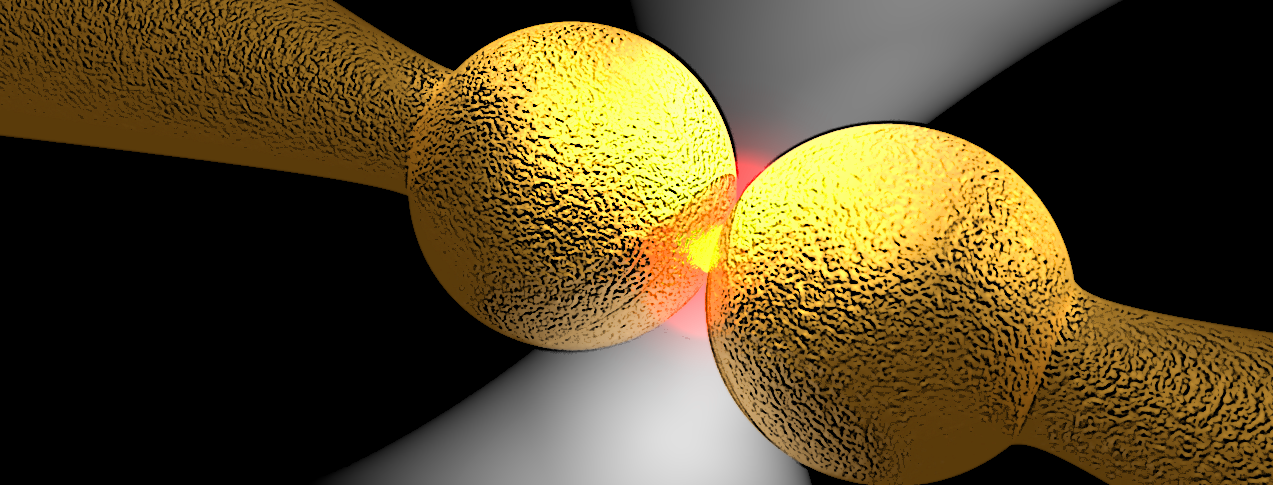
\includegraphics[width=\paperwidth]{../chapter_covers/tip_interactions_cover.png}}
\put(415,-30) {\begin{minipage}{0.35\textwidth}\flushright\singlespace\fontsize{9pt}{1em}\selectfont\color{white} Graphical representation of the spherical Au tip dimer used to investigate plasmon coupling in the quantum regime.\end{minipage}}
}}

The final set of experiments discussed in this thesis are the product of each of the developments from previous chapters, utilising pairs of tips in the microscope platform to investigate the limits of plasmon coupling. Coupling between different tip morphologies is dynamically investigated to both confirm plasmonic behaviour in tips and increase understanding of the characteristic regimes of plasmon coupling, including the recently uncovered quantum regime. Through this work an improved interpretation of future results in sub-nm plasmonic gaps can be attained.

\subimport{./}{tip_dimer_interactions}
\subimport{./}{quantum_effects}

\section{Conclusions}

Multiple different combinations of tips in a dimer configuration are used to probe plasmon coupling. Sharp Au tips exhibit no obvious plasmon resonances under far-field illumination and no gap mode coupling is observed with other sharp or spherical Au tips. This is caused by the lack of an antenna-like geometry in sharp tips. Plasmons excited at the apex of spherical Au tips, on the other hand, interact and form coupled modes. The behaviour of these modes is as expected, with similarity to plasmons in AuNP dimers. The inherent asymmetry between the large spherical tip structures leads to more complex scattering spectra wherein anti-bonding modes are no longer dark. Their spatial evolution into gap modes is something not previously seen before within a single plasmonic system.

To conclude experimental work, tip dimers are used to investigate the quantum regime of plasmonic coupling, specifically the effects of quantum charge transport. Using this approach, the development of the quantum regime is dynamically observed. Critical conductances are estimated for the onset of each characteristic effect using direct correlations between optical spectra and current measurements. Measurements agree well with theoretical principles. Though no quantitative measurements, such as temperature, voltage or power dependences, are made to guarantee the exact mechanisms of charge transport, quantum tunnelling and ballistic conductance are the most likely mechanisms. Further investigation could quantify this, although charge transfer phenomena are not expected to depend on the specific conduction mechanism. Comparison with tip dimers coated in different molecular layers of varying conductivities would add further understanding into the effects of charge transfer and forms the basis of future experiments on this topic.

In summary, the existence of two distinct regimes of quantum charge transport have been detected in sub-nm plasmonic cavities. These are:
\begin{itemize}
\item The tunnelling regime (also known as the crossover regime), wherein electrons tunnelling through the gap barrier screens the local capacitive interaction between opposite gap surfaces, reducing plasmon coupling strength and slowing the associated redshift to a halt.
\item The conductive regime, where strong currents at \G0-level conductances heavily attenuate gap plasmons and lead to the previously observed blueshift transition into charge transfer plasmons.
\end{itemize}
Though numerous theoretically predictions and experiments have been reported in recent years, this is the first time that correlated experimental measurements between plasmon resonances and conductance have been performed to understand quantum effects in plasmonic systems.

\ifstandalone
\begin{singlespace}
\fontsize{8pt}{1em}\selectfont
\printbibliography[notcategory=fullcited]
\end{singlespace}
\fi

\end{document}